\section{Prototypes, Sketches, Studies}

  \subsection{Methodology}
  
    \subsubsection{Design Process Approach}
      \begin{figure}[H]
        \centering
        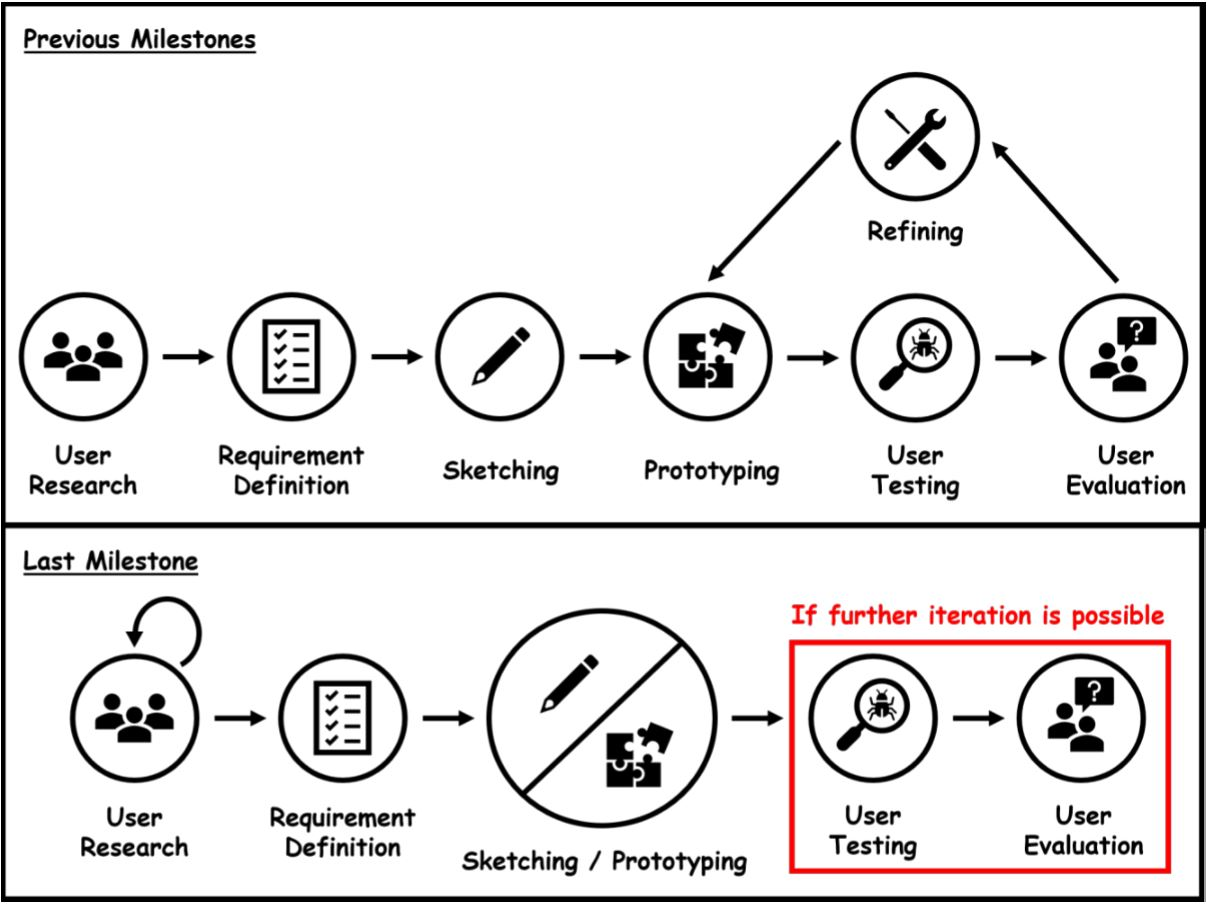
\includegraphics[width=\textwidth]{img/prototype/prototype-1.JPG}
        \caption{Prototype Design Approach}
        \label{fig:design-approach}
      \end{figure}
      \par \textbf{Summary}:
      \par As shown in figure \ref{fig:design-approach}, our approach for the previous milestones (iteration 1 and 2) were focusing
      more towards the implementation of designing and refining features based on how the users
      responded throughout the user testing session. With this approach, we had realized that refining the
      prototype specifications to display features that satisfy the users does not aligned with the initial
      concepts and goals we want to deliver as an application that deals with a pandemic outbreak situation.
      \par During the interim presentation with our peers and mentors, we received critiques of our proposed
      application does not have a core value to deliver to the stakeholders. After realizing what we are
      lacking, we revamp our design approach to specify our core values that the application should be
      delivered. With getting user inputs that is based on our application core values, we can illustrate a
      better prototype that satisfy the users with the prerequisite of fulfilling the core goals. As there are
      time constraints for the last milestone (iteration 3), we could only manage to proceed until the
      prototyping phase. Any user testing and evaluation can be done if there is any further iterations.

    \subsubsection{Terminology}
      \begin{itemize}
        \item \textbf{User Research}
          \par User research is to create assumptions for features that are necessary and crucial for the product user. It helps to create user personas for the target audience through representations of their demographics, habits and behaviour patterns. Various data collection methods are used to collect information in an iterative breadth-and-depth approach.
        \item \textbf{Requirement Definition}
          \par The information collected are analysed to discover insights for involving quality features for the target
          audience. Hence, information can be compiled to create specific product requirements with proper
          documentation. The documentation would be the overview and detailed description of the methods
          used to create the prototype of our problem space with delivering our core values.
        \item \textbf{Sketching}
          \par Sketching helps to visualizing features or the product contents to present how the illustrated
          components could help the users to achieve their goals upon using the product. It is to provide the
          best possible user experience with visual components and draft segments. It is encouraged to receive
          continuous feedbacks from users of the target audience for better visual input if possible. However,
          our last milestone (iteration 3) could only focus on creating the prototype through delivering our core
          values without further testing user input.
        \item \textbf{Prototyping}
          \par An interactive model of the product is created with integrating suitable visual components. The
          prototype could be developed with multiple iterations through collecting feedbacks during usability
          testing if possible. Despite that, we focused on creating a high-level prototype that deliver our core
          values on the last milestone (iteration 3) only due to time constraint.
        \item \textbf{User Testing}
          \par Usability testing is conducted with end users of the target audience consisting of probing or think-
          aloud techniques and A/B testing for collecting user inputs. Various testing techniques will be
          explained below with more descriptive examples and statements. User testing is not being carried out
          in the last milestone (iteration 3). Any further iterations could perform user testing if possible.
        \item \textbf{User Evaluation}
          \par Product analytics could be made with analysing and evaluate the user inputs upon the product for
          assessing the product potential. These inputs are studied for design and usability optimization. There
          is no evaluation as user testing is not carried out in the last milestone (iteration 3).
        \item \textbf{Refining}
          \par Prototype refinement made through iterative and incremental process after user evaluation. This step
          is removed in the last milestone (iteration 3) as our team has created a goal to deliver the core values
          with an initial design for the prototype. Any further research could be carried out by another team.
      \end{itemize}

  \subsection{Research Study}
    \subsubsection{Data Collection Methods}
      \begin{enumerate}[a)]
        \item \textbf{Iteration 1}
          \begin{itemize}
            \item \textbf{Surveys}
              \par Survey is a method of quantitative research. It is used as an approach for collecting a more structured
              and statistical data for general background study. The participants were from various age groups as
              there is no conditional user restrictions, the possible solution is to cater all age groups. Thus, collected
              responses are used for further evaluation to create a solution for general users. Moreover, this is a
              crucial process to understand the requirements for system visualization during design planning. The
              survey was designed through Google Form and made available online. The responses are attached
              below in Appendix \ref{appendix:survey}.
              \par \textbf{Findings}
              \begin{itemize}
                \item Based on figure \ref{fig:findings-1}, approximate 33\% of the respondents do not trust the data being protected
                regardless of it being a third-party or the government.
                \item Based on figure \ref{fig:findings-2}, 60\% of the respondents thinks that a contact-tracing application would be useful.
                \item Based on figure \ref{fig:findings-3}, approximately 73\% of the respondents turn on the location service feature which
                around 80\% gives location access only when the application request from the users.
              \end{itemize}
              \begin{figure}[H]
                \centering
                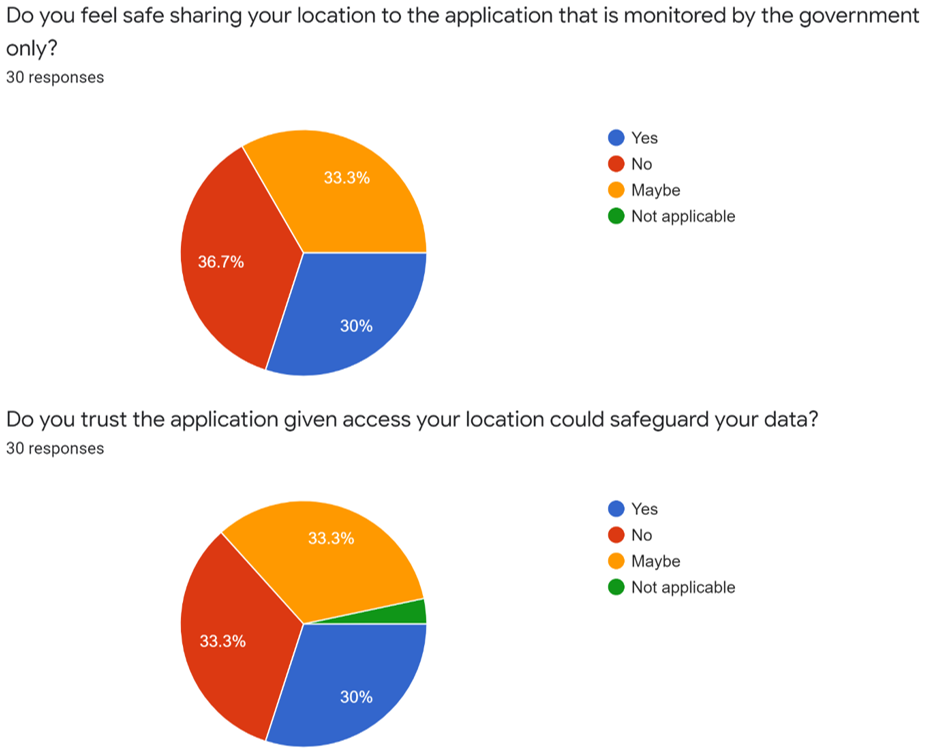
\includegraphics[width=\textwidth]{img/findings-1.png}
                \caption{Questions on Government Credibility to Safeguard Data}
                \label{fig:findings-1}
              \end{figure}
              \begin{figure}[H]
                \centering
                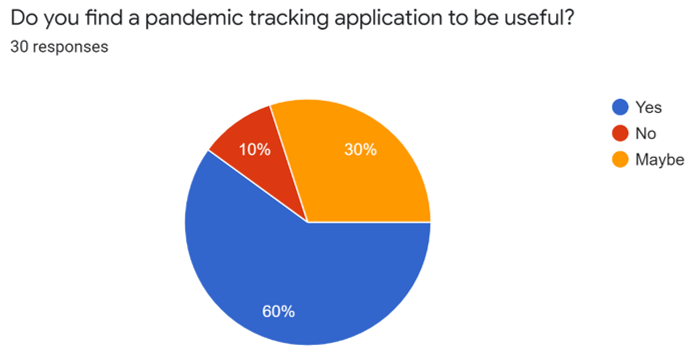
\includegraphics[width=14cm]{img/findings-2.png}
                \caption{Question on Usefulness of Pandemic Application}
                \label{fig:findings-2}
              \end{figure}
              \begin{figure}[H]
                \centering
                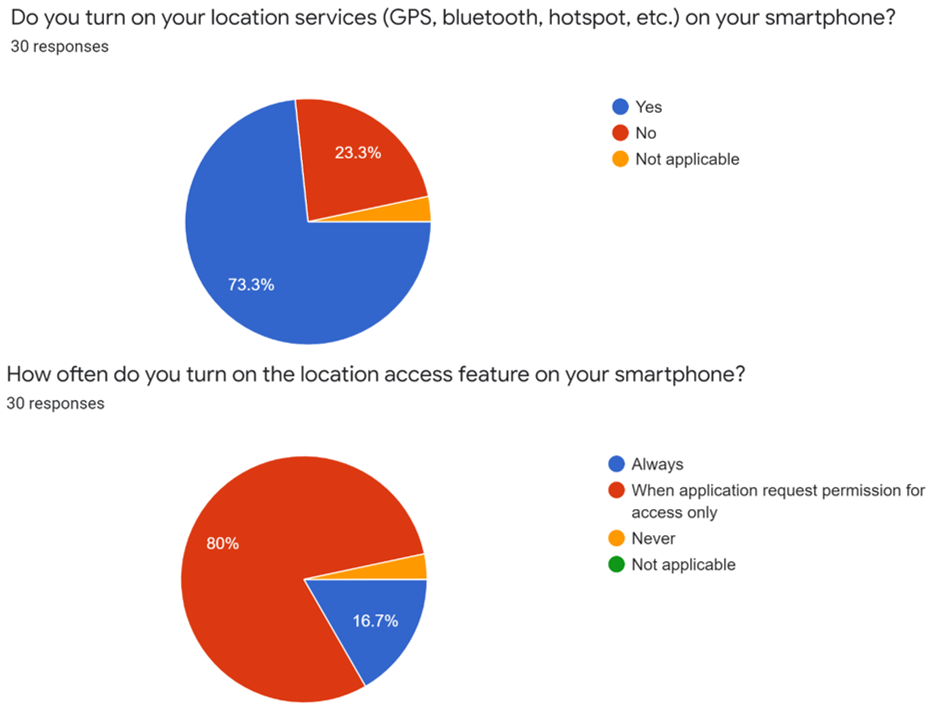
\includegraphics[width=\textwidth]{img/findings-3.png}
                \caption{Questions on User Usage on Mobile Location Access Feature}
                \label{fig:findings-3}
              \end{figure}

            \item \textbf{Interviews}
              \par Interview is a method of qualitative research. It is used as an approach for collecting descriptive
              opinions and views among specific users in different user categories. The list of interviewees was
              focused upon 3 different age groups consists of a primary school student, a young adult retail worker,
              and a retired elderly that represents the age ranges of 0 to 17, 18 to 64, and above 65 respectively.
              The interview is composed of designed questions based on the evaluation from the survey, follow-up
              questions may also be included to gather more in-depth data. Thus, this helps to discover information
              based on their thinking, attitudes and even motivations. All interviewees have expressed consent to
              participate in this research study. The interviews were all conducted through online video call. The
              transcripts are attached below in Appendix \ref{appendix:interview}
              \par \textbf{Findings}
                \begin{itemize}
                  \item Minors do not think the application is necessary for them.
                  \item Most adults are concerned with application using location sharing.
                  \item Accessibility features implementation is a concern for elderly community that include disable individuals.
                \end{itemize}
            \item \textbf{Insights}
              \begin{itemize}
                \item The number of application users could directly be influenced with the habit of users utilizing the location services or not, as it is necessary for the application to use the location services feature.
                \item Most participants do not trust any application that always collects their location data.
                \item Most participants are doubtful of the government credibility in protecting their data.
                \item Parental guidance and control could be a reason for minors not finding the application useful.
                \item Increasing accessibility features for accommodating user groups with disability could create a higher acceptance among the elderly or disable community.
                \item Proper digital privacy establishment is necessary for users to trust the application provider in handling their data.
              \end{itemize}
          \end{itemize}
        \item \textbf{Iteration 2}
          \begin{figure}[H]
            \centering
            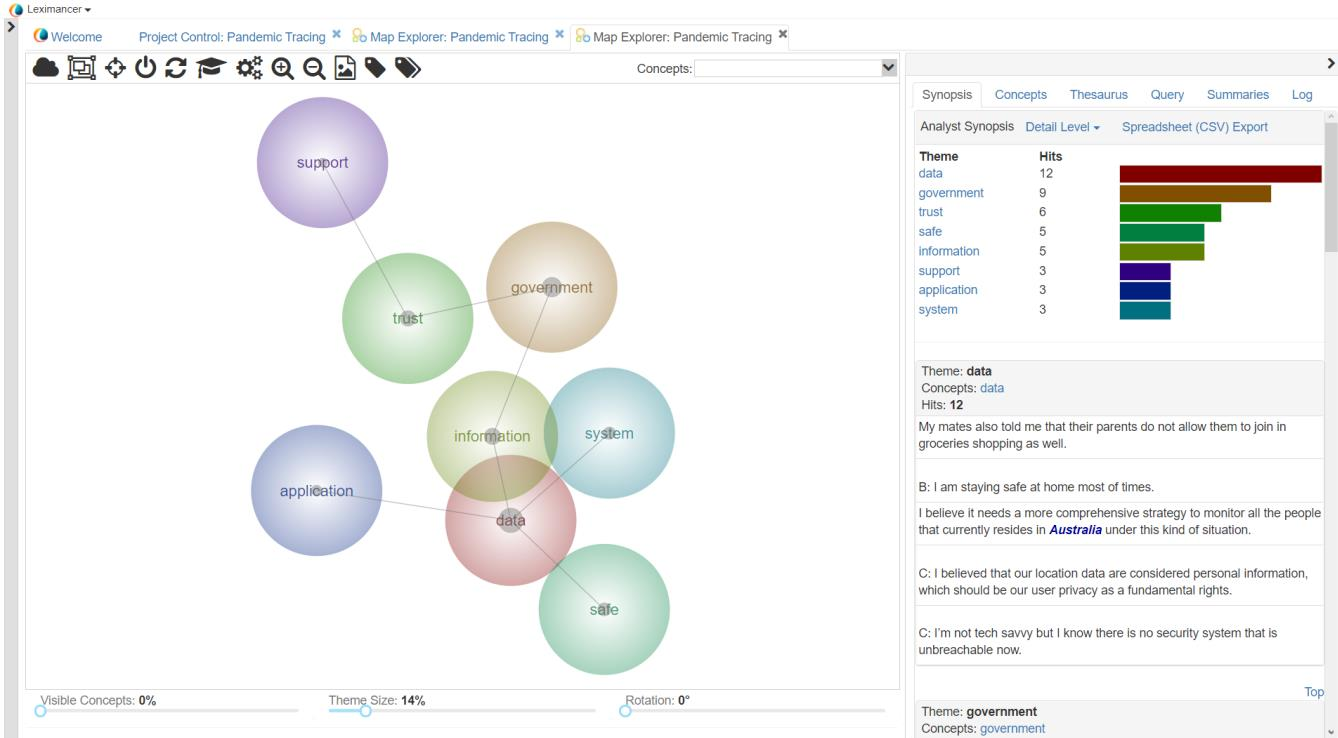
\includegraphics[width=\textwidth]{img/prototype/lexi.png}
            \caption{Text Clustering Analysis from Iteration 1 Interviews}
            \label{fig:findings-2}
          \end{figure}
          \begin{itemize}
            \item \textbf{Additional analysis}
              \par During Iteration 2, a text clustering was performed for the interview transcript generated during the previous milestone (Iteration 1). Text clustering is an application of cluster analysis for textual documents. It allows grouping for different set of unlabelled words with similarity within in the same cluster. Hence, this approach could further find insights from keywords mentioned from the interviews to further provide guidance for better decision making and define our project goals.
              \par Our approach to use text clustering includes the reasoning of lacking at least a core value for our product that should delivers to the target audience. With using this approach, we can identity some keywords mentioned many times such as ``support and ``trust" along with the previous survey insights generated from the previous milestone (Iteration 1) and further consolidate it to create our goals that identifies the core values we want to deliver to the stakeholders as a pandemic tracking application.
          \end{itemize}
        \item \textbf{Iteration 3}
          \begin{itemize}
            \item \textbf{Surveys}
              \par As our team also realized how important data privacy should be considered during surveys while
              collecting data, all the involved participants ID will be masked and anonymized. The survey question
              would be related to our core goals and values that our application would like to deliver. The
              participants were mostly from the same group of the previous milestones (iteration 1 and 2). The
              survey was designed through Qualtrics and made available online. The responses are attached below
              in Appendix \ref{appendix:iter3-survey}.
                \begin{figure}[H]
                  \centering
                  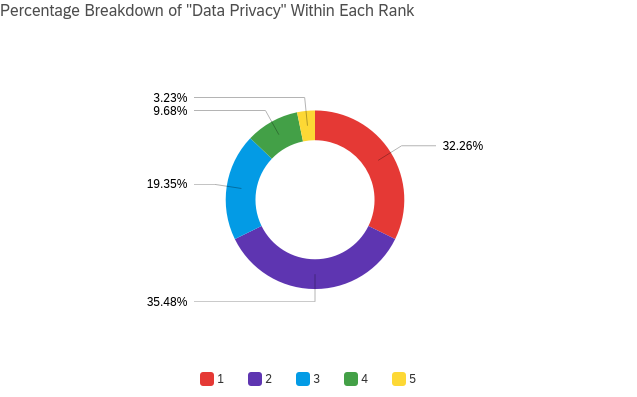
\includegraphics[width=\linewidth]{img/prototype/iter3-survey-findings-1.png}
                  \caption{Data Privacy Overall Ranking}
                  \label{fig:iter3-survey-findings-1}
                \end{figure}
                \begin{figure}[H]
                  \centering
                  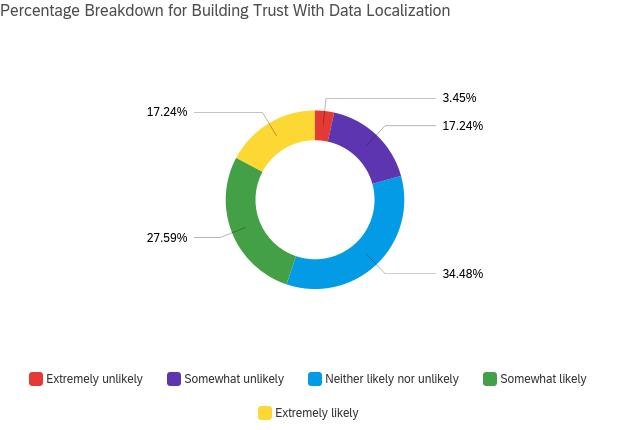
\includegraphics[width=\linewidth]{img/prototype/iter3-survey-findings-2.png}
                  \caption{Total Percentage Distribution of Building Trust with Data Localization}
                  \label{fig:iter3-survey-findings-2}
                \end{figure}
                \begin{figure}[H]
                  \centering
                  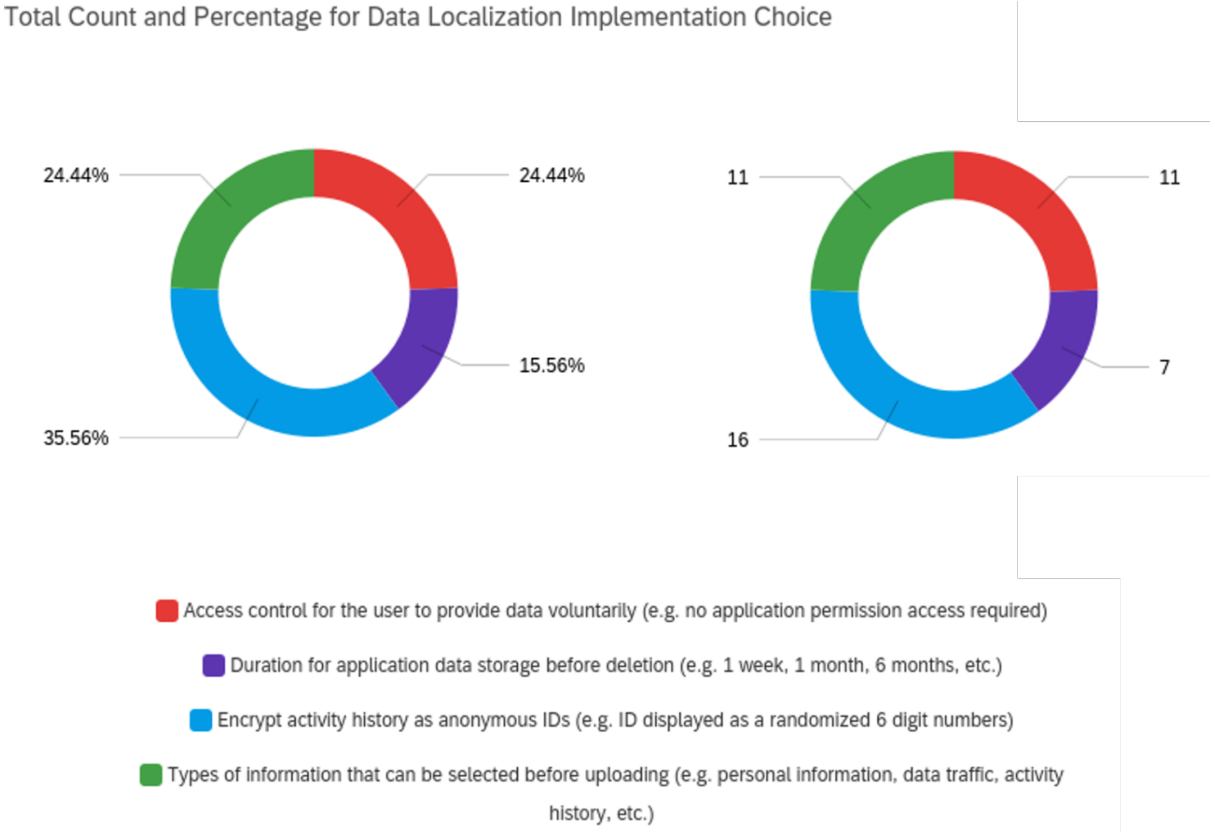
\includegraphics[width=\linewidth]{img/prototype/iter3-survey-findings-3.png}
                  \caption{Total Distribution of Count and Percentage for Data Localization Implementation}
                  \label{fig:iter3-survey-findings-3}
                \end{figure}
              \par \textbf{Findings}
              \begin{itemize}
                \item Based on figure \ref{fig:iter3-survey-findings-1}, respondents have rank data privacy as the top 1 and 2 priority in a mobile
                application which are approximately 32\% and 35\% respectively.
                \item Based on figure \ref{fig:iter3-survey-findings-2}, approximate 44\% of the respondents think that mobile application that implement
                data localization could build trust with the user.
                \item Based on figure \ref{fig:iter3-survey-findings-3}, the top 3 implementation choices chosen by the respondents include anonymous
                ID, access control for voluntary data upload and type of data upload which are 35\%, both 24\%
                respectively.
              \end{itemize}
              \par \textbf{Insights}
              \begin{itemize}
                \item Data privacy has proven to be an important factor for a mobile application throughout both survey
                sessions by similar respondent groups.
                \item Data localization could be a good concept to build trust with user for mobile application that
                requires data sharing.
                \item The choices chosen by the respondents for data localization implementation are closely aligned
                and related with our core values of the proposed application.
              \end{itemize}
          \end{itemize}
      \end{enumerate}

  \subsection{Sketches}
    \subsubsection{Simulation}
      \begin{enumerate}[a)]
        \item \textbf{Iteration 1}
          \begin{figure}[H]
            \centering
            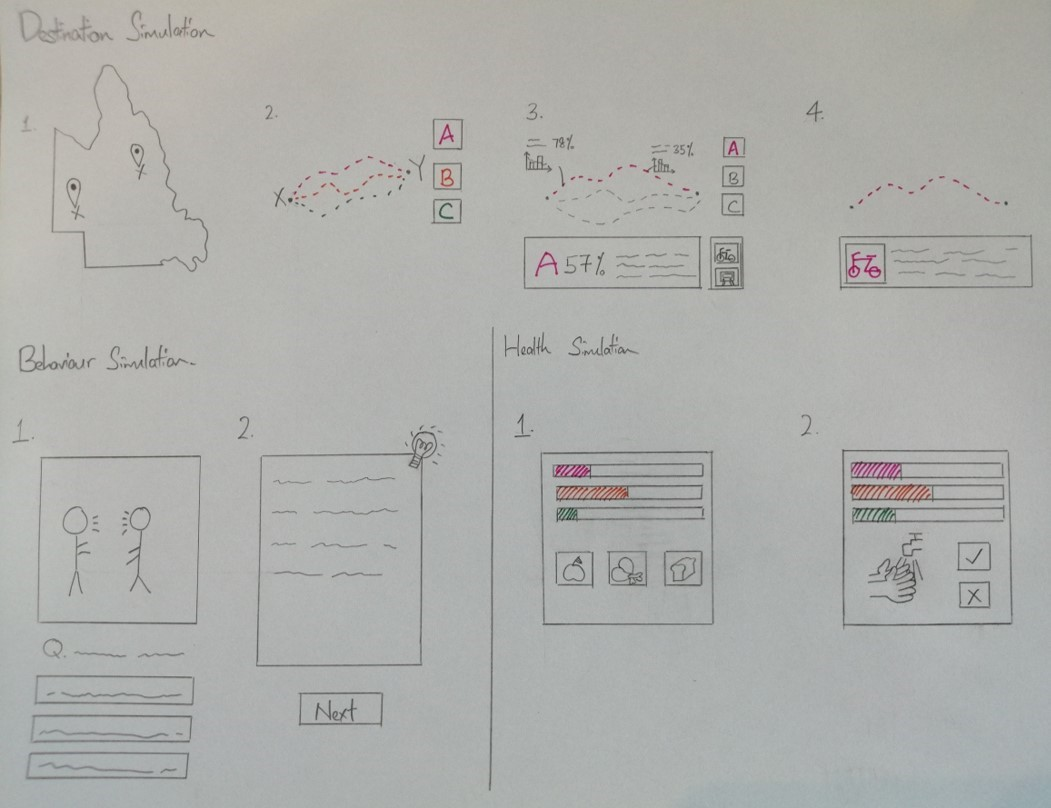
\includegraphics[width=\linewidth]{simulation.jpg}
            \caption{Simulation Sketches}
            \label{fig:simulation}
          \end{figure}
          \par Based on figure \ref{fig:simulation}, various simulations are considered during the first iteration. The sketches will be designed and showcased digitally to be interactable as a feature implementation for the proposed solution during the second iteration. The purpose of a simulation is to provide a learning opportunity for the users. Furthermore, it promotes the application to be more educational through a human-computer interaction (HCI) design. Moreover, this will increase the user flow whenever the user interacts with the simulation, which creates possibility of more user scenarios in a simulated environment with real-life aspects during pandemic outbreak. In addition, it provides a pleasant user experience when information is conveyed via gamification with audio and visual components. Hence, the information conveyed by the simulations to the user helps to deliver the values of the application. The simulation works with navigating the user through a journey that is projected with real-word aspects by embedding and implicit impressions which may turn into healthy habits and matured practices. In other words, it encourages habit and behaviour changes when appropriate information is conveyed in an interactive manner that could be instilled into users under these special circumstances.
        \item \textbf{Iteration 2 and 3}
          \par There are no sketches created for the third iteration. As sketches are harder to illustrate the user
          scenario process of how data localization is implemented in our proposed solution. Our team decided
          to proceed with presenting the visual design through digital prototyping. The reason is due to the
          approach of digital prototyping could provide higher level in clarity for describing the user scenario
          process of specific situations that showcase the functionalities.
      \end{enumerate}

  \subsection{Prototypes}
    \subsubsection{Constrained Prototyping}
      \par Business Model Canvas is a method for constrained prototyping. The aim of a business model canvas is to explicit the values of the product through aligning various key elements during design planning phase. It provides a clear information outline for creating wireframe elements. Furthermore, it helps to visualize the conceptual idea of delivering a minimum viable product (MVP) which could serve as the basic form for the prototype.

      \par The canvas shown below in Figure \ref{fig:bmc} defines the general scope with descriptive points within the key elements section.

      \begin{figure}[H]
        \centering
        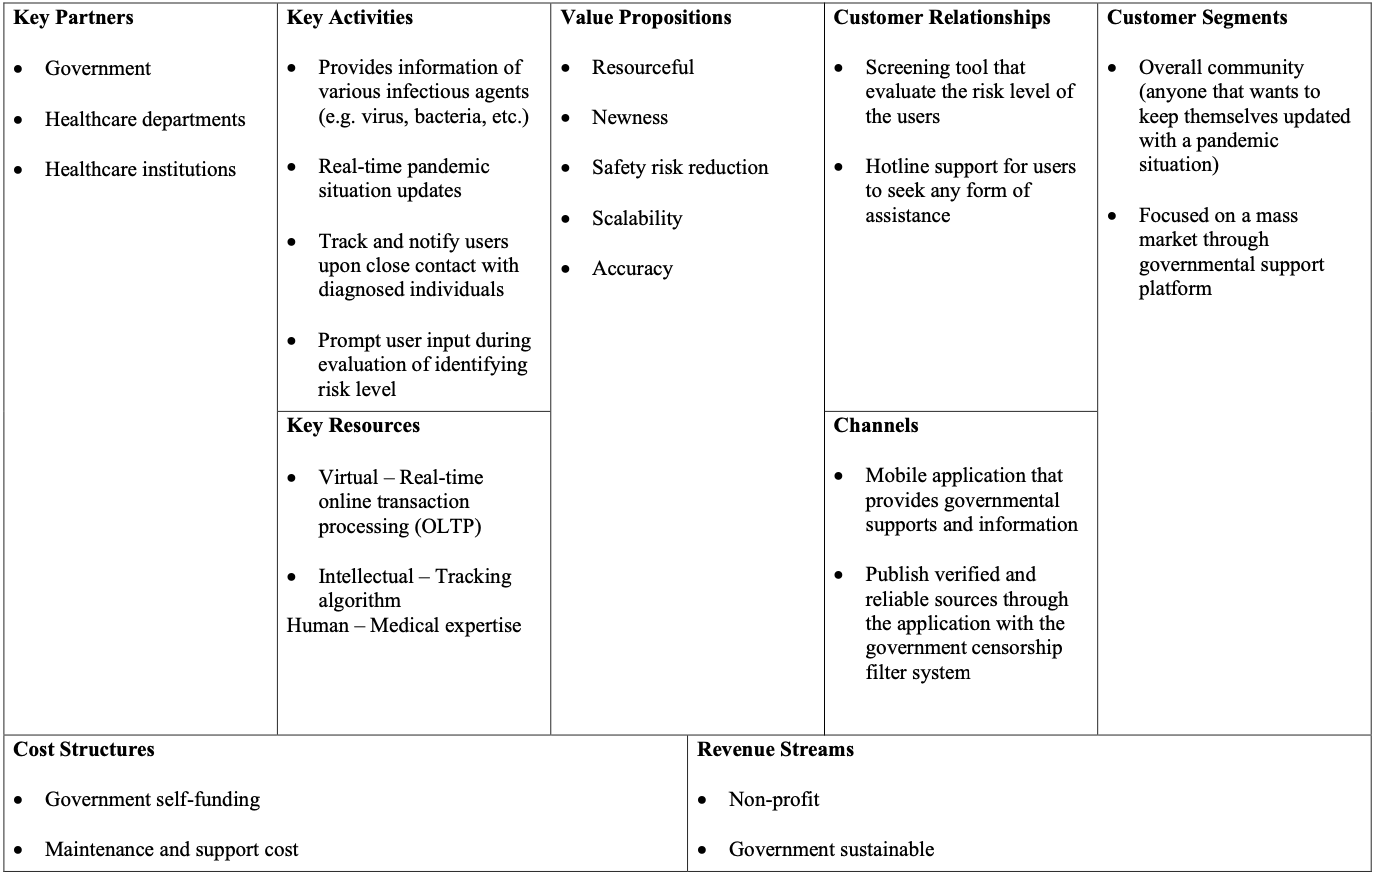
\includegraphics[width=\linewidth]{img/bmc.png}
        \caption{Business Model Canvas}
        \label{fig:bmc}
      \end{figure}
    
    \subsubsection{Paper prototyping}
      \par This approach is a method to quickly visualize the conceptual designs that could be a wireframe for
      the digital interfaces. A total of 9 simple interfaces of low-fidelity wireframes were created to
      showcase the general functionalities through the proposed solution interfaces.
      \begin{figure}[H]
        \centering
        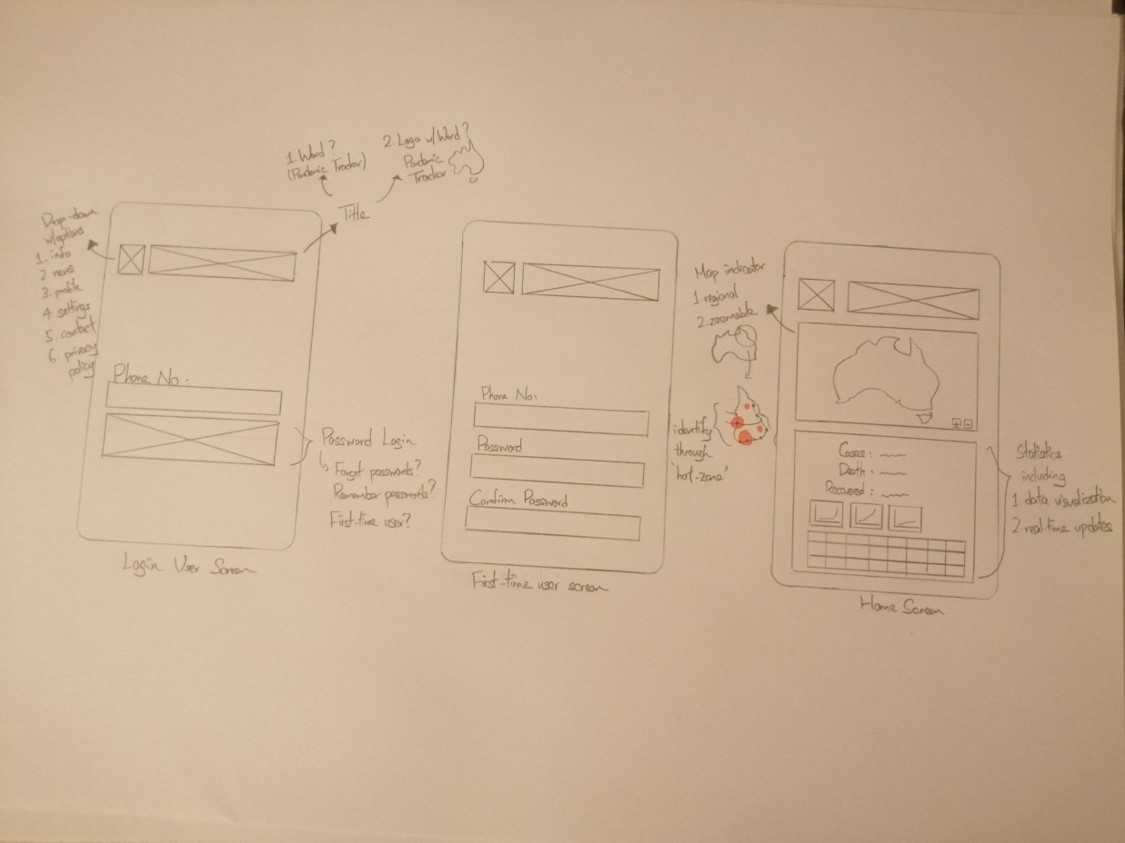
\includegraphics[width=\linewidth]{img/low-fidelity-prototype/sketch-1.png}
        \caption{Login, Register and Home Screen}
        \label{fig:prototype-01}
      \end{figure}
      
      \par Based on Figure \ref{fig:prototype-01}, the wireframe consists of the login, register and home screen interfaces, A valid phone number and a password is required for login. For first-time user, the login screen will have a link directing the user to the register screen to fill in the phone number and password to register as a member. Account recovery methods such as password reset will be included if the users forget their password. The home screen would include a heatmap indicator with statistical data of regional information including zone safety level, statistics, distribution of cases (orange dots in colour).
      
      \begin{figure}[H]
        \centering
        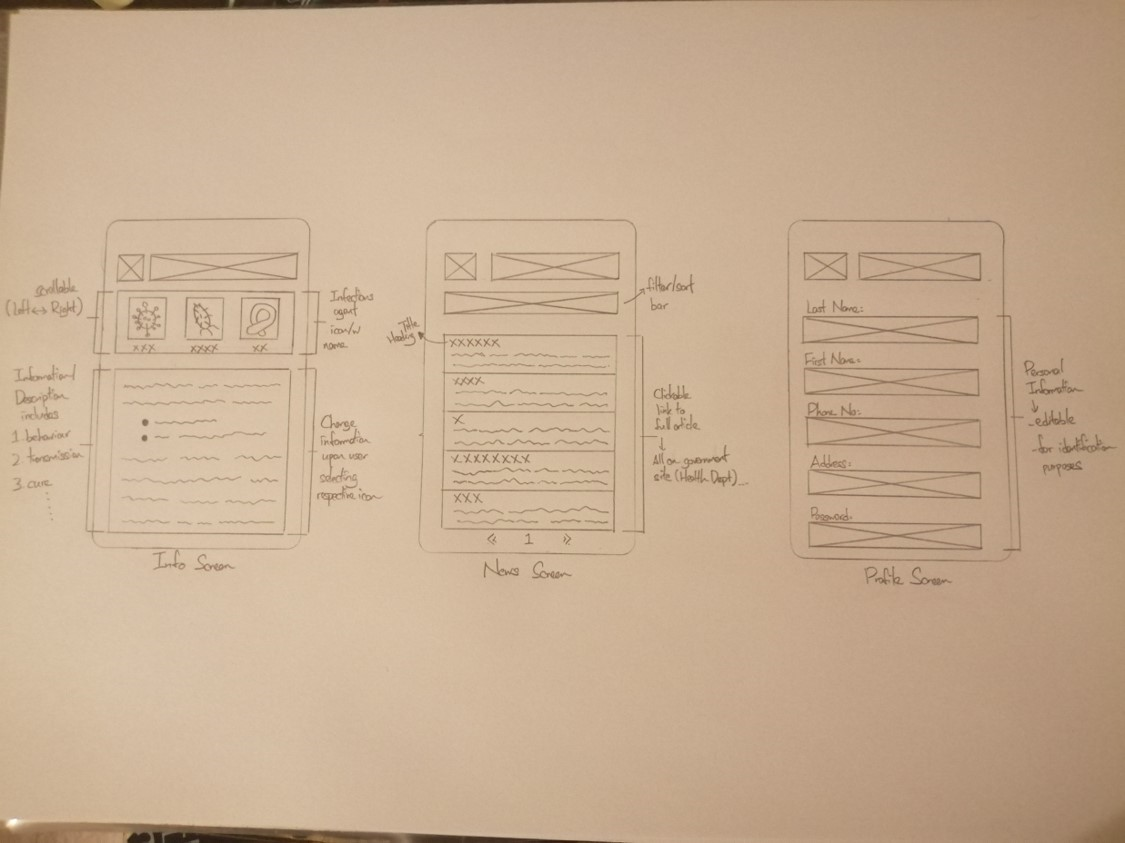
\includegraphics[width=\linewidth]{img/low-fidelity-prototype/sketch-2.png}
        \caption{Info, News and Profile Screen}
        \label{fig:prototype-02}
      \end{figure}

      \par Figure \ref{fig:prototype-02} shows the information, news and profile screen. Basic information of the infectious agents will be explained in layman terms which includes behaviour, characteristics, transmission and more. The following news screen are latest updated articles from verified publishers for any international and domestic news. The profile screen will display basic information consists of the authentic name of the user, phone no, and home address, which is crucial when immediate quarantine or government support is needed.

      \begin{figure}[H]
        \centering
        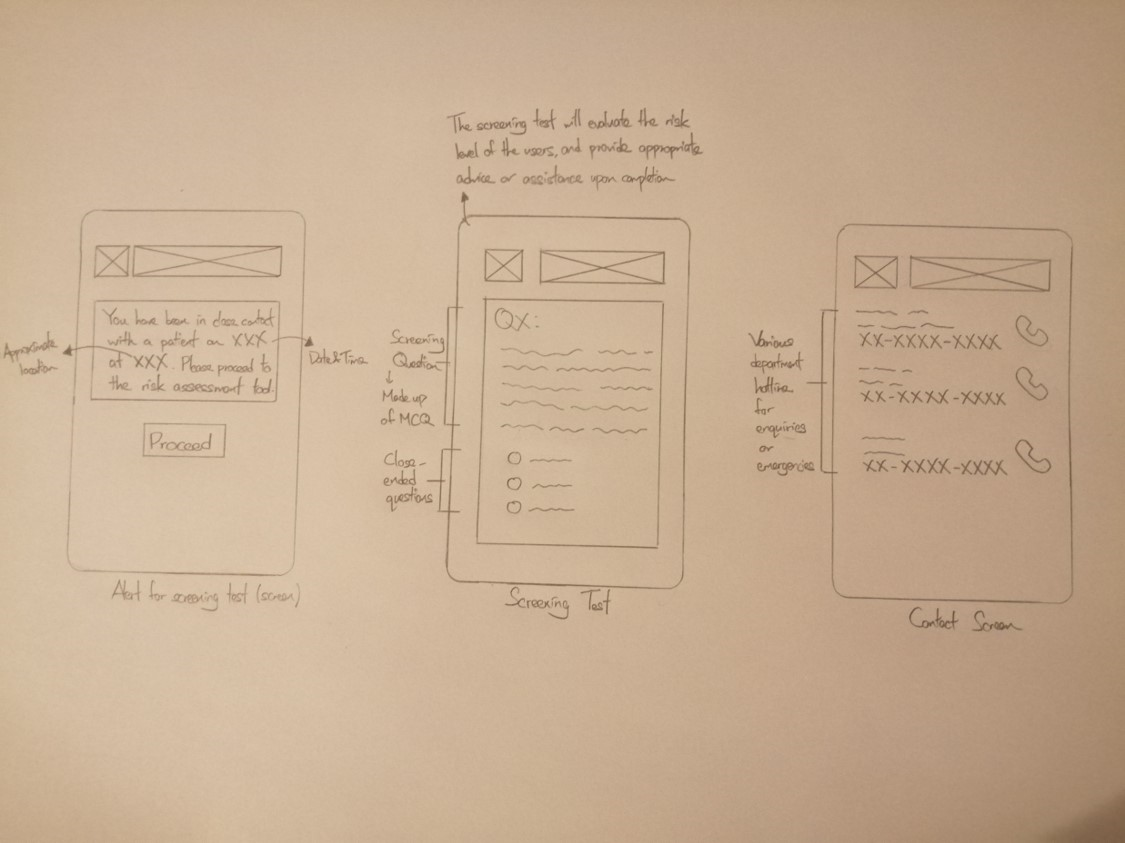
\includegraphics[width=\linewidth]{img/low-fidelity-prototype/sketch-3.png}
        \caption{Notification, Q\&A and Contact Screen}
        \label{fig:prototype-03}
      \end{figure}
      
      \par An alert notification, screening test and contact screen is shown in Figure \ref{fig:prototype-03}. The alert notification would pop up when the user has been verified having close contact with a diagnosed individual. The user will then be prompted to proceed to the Q\&A panel for a short evaluation. The result will display the user's personal risk level, which may or may not necessarily to request medical support. Apart from this, the contact screen is listed with relevant government hotlines that could be helpful for enquiries or emergencies directly.

    \subsubsection{Digital Prototyping}
      \par This approach is to create a high-fidelity sketch for multiple user interfaces. A wireframe is built upon
      a mixture of simulations contents with including basic design components. The current digital
      prototypes do not focus on the main functionalities of how a pandemic tracking application should
      operates. However, it focused on finding elements and concepts that could be included by studying
      user behaviour through usability testing to increase adoption and retention rate of the application.

      \begin{enumerate}[a)]
        \item \textbf{Iteration 2}
        \begin{enumerate}[label=(\roman*)]
          \item \textbf{Map Simulation}
            \begin{figure}[H]
              \centering
              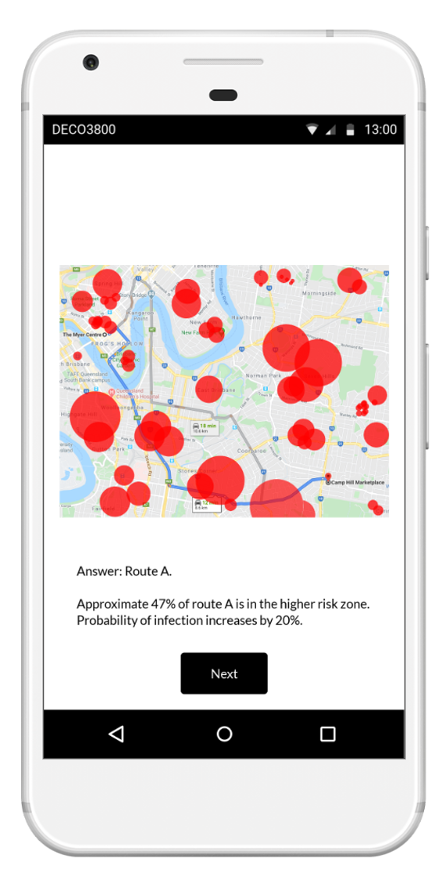
\includegraphics[scale=1]{img/digital-prototype/map-simulation.png}
              \caption{Map Simulation}
              \label{fig:digi-proto-01}
            \end{figure}
            \par The above Figure \ref{fig:digi-proto-01} simulation was proposed as a part of the product goals to improve decision making in risk assessment during travelling. Moreover, this simulation is integrated with the real-time heat map generated from the COVID-19 statistics. This algorithm will be included to calculate the user infection rate throughout the planned journey which happen to be in the hot zone when travelling.
            \par This simulation could act as a supplementary tool for helping user to make sound judgement to considers their surrounding loved ones as well. This could also invoke empathy among the users and therefore encourages it for journey planning. Thus, helping user to build a stronger relationship with their loved ones among this pandemic period.
          \item \textbf{Quarantine Life Simulation}
            \begin{figure}[H]
              \centering
              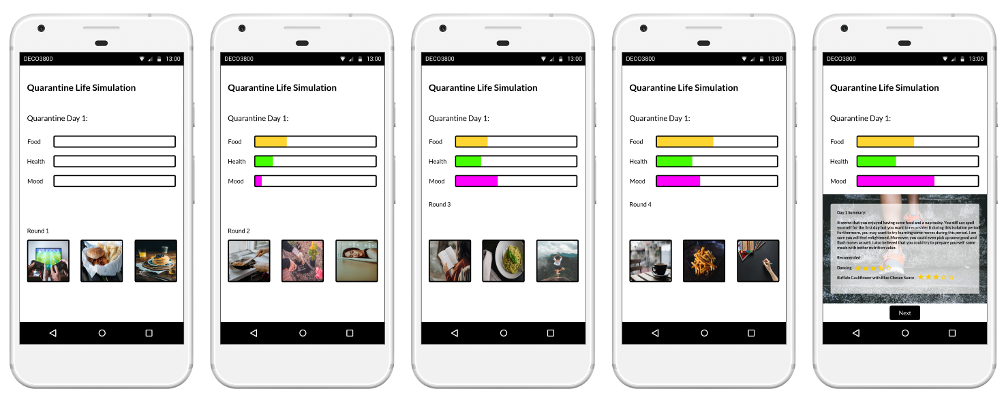
\includegraphics[scale=1]{img/digital-prototype/quarantine-life.png}
              \caption{Quarantine Life Simulation}
              \label{fig:digi-proto-02}
            \end{figure}
            \par The above Figure \ref{fig:digi-proto-02} simulation through cognitive learning was proposed as a part of the product goals to promote a healthier lifestyle during this pandemic period. Moreover, this simulation implemented via gamification through selecting a desire picture through each round daily. The food, health and mood barometers are each an attribute representation of eating habits, vitality and mental state. The system will then analyse the user behaviour and provide a summary according to the user selection including the total percentages in the barometers. The summary will include user the behavioural pattern and provide recommendations to improve certain attributes. Hence, this simulation could help encourages habits and behaviours change during this pandemic period for user to adopt a healthier lifestyle for low stress living.
          \item \textbf{Simulations Removal}
            \par In the final presentation for Iteration 2, our team receive critiques from the mentors and peers regarding the obscurity of our product positioning as a pandemic tracking application. As our goals set were trying to include more features in other aspects such learning with how the typical pandemic tracking applications (e.g. Australia COVIDSafe, Singapore TraceTogether) did not provide, it was more of a benefit-focused positioning for the product. However, after we realize how both COVIDSafe and TraceTogether has not been very successful through in-depth research, we found out there is a barrier for users to ``trust" their data and privacy with us. Hence, we changed our product goals approach that is a behaviour-based positioning. With this approach, we focused on building trust with users that the application may evoke such a feat to increase user participating and engaging with application. In other words, we do not further include educational simulations which are not aligned with our product goals that deliver the core value of building ``trust" with the user.
        \end{enumerate}
        \item \textbf{Iteration 3}
          \par The below figures will display the functionalities of our final proposed solution to deliver the core
          values as a pandemic tracking application.
          \begin{figure}[H]
            \centering
            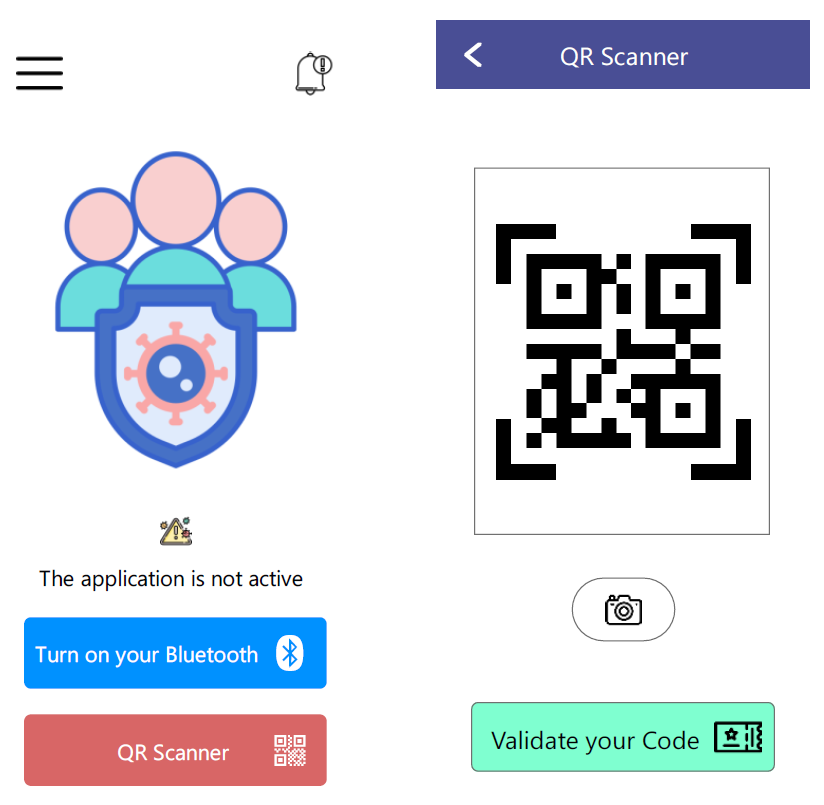
\includegraphics[scale=1]{img/prototype/iter3-proto-1.png}
            \caption{Main Screen and QR Code Scanner Screen}
            \label{fig:iter3-proto-1}
          \end{figure}
          \par According to figure \ref{fig:iter3-proto-1}, the left screen displayed the two main functionalities of the application, which
          are the Bluetooth status and the QR Scanner. If the Bluetooth is deactivated, a button with be
          prompted with a message ``Turn on your Bluetooth" that will direct the users to the Settings screen to
          activate it once pressed. Besides that, while being at outdoors, the users would need to scan the QR
          Code to access certain areas or zones through tapping on the ``QR Scanner" button. After that, a screen
          shown as the right of figure \ref{fig:iter3-proto-1} will provide the users with two options, either by scanning the code via
          camera or authenticating the scanned code validity via the ``Validate your Code" button.
          \begin{figure}[H]
            \centering
            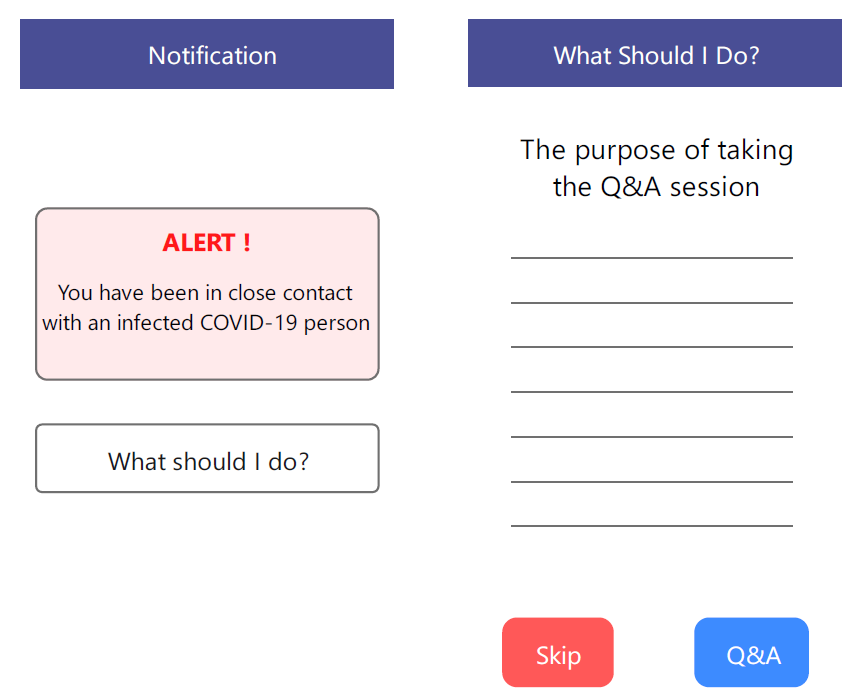
\includegraphics[scale=1]{img/prototype/iter3-proto-2.png}
            \caption{Notification and Screening Test Guideline Screen}
            \label{fig:iter3-proto-2}
          \end{figure}
          \par Based on figure \ref{fig:iter3-proto-2}, the left screen displayed a message notifying the user when had been close contact
          with a positively tested individual. The notification system is one of the core features that the
          application delivers its core values to the user. The user could only navigate to the right screen shown
          in figure \ref{fig:iter3-proto-2} through tapping on ``What should I do?" button. It will then allow the user to know more
          about the purpose of proceeding with the Q\&A session to receive advices from the health authorities.
          However, the user has the options whether to proceed or not either ignoring it by tapping the skip
          button or proceeding the session by the Q\&A button. The user can still access to the right screen of
          figure \ref{fig:iter3-proto-2} via the notification icon on the top left corner of figure \ref{fig:iter3-proto-1} left screen.
          \begin{figure}[H]
            \centering
            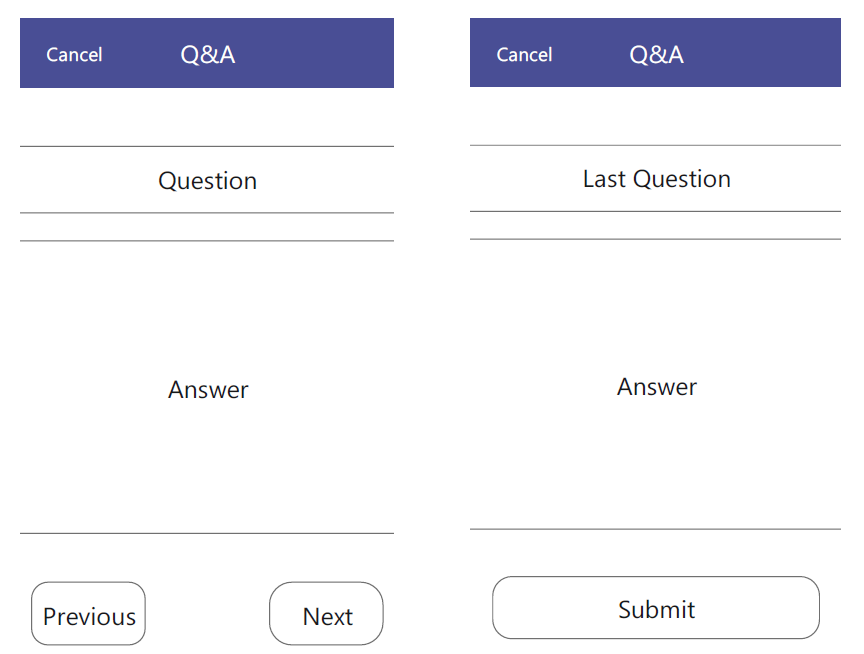
\includegraphics[scale=1]{img/prototype/iter3-proto-3.png}
            \caption{Notification and Screening Test Guideline Screen}
            \label{fig:iter3-proto-3}
          \end{figure}
          According to figure \ref{fig:iter3-proto-3}, the left screen is the screening test screen after the user agreed to participate in it by tapping the Q\&A button in the right screen of figure \ref{fig:iter3-proto-2}. The screening test consist of several questions without any questions that needs any demographic and geographic information input by the user. A user can decide to opt-out the test anytime via the ``Cancel" button on the top-left corner of figure \ref{fig:iter3-proto-3} left screen. Moreover, the user could skip any questions through the ``Next" button and navigate to the previous question through the ``Previous" button. The right screen of figure \ref{fig:iter3-proto-3} is the submit screen for the screening test. The user could complete the test by tapping on the ``Submit" button. All the data is then recorded and redirects back to the main screen.
          \begin{figure}[H]
            \centering
            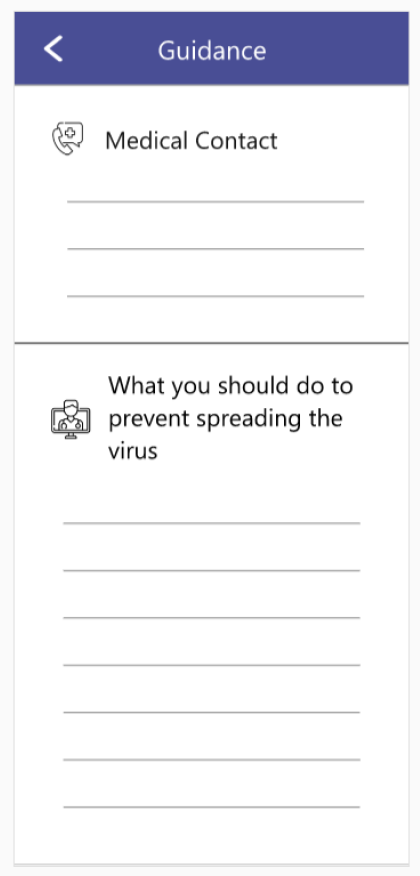
\includegraphics[scale=1]{img/prototype/iter3-proto-4.png}
            \caption{Support Screen}
            \label{fig:iter3-proto-4}
          \end{figure}
          Based on figure \ref{fig:iter3-proto-4}, it is a support screen that provides numerous support channels to guide and help any users in need. The User Guidance screen would include essential categories such medical contacts and prevention measures. If a user needs a list of emergency and health support hotlines, they could tap on the Medical Contact section. The purpose of this implementation is to provide users a readily accessible way to receive the support they need. Moreover, if the users are unsure how to keep themselves protected and prevent further transmission of the virus, they could explore the suggestions section that provides detailed instructions for the prevention measures.
          \begin{figure}[H]
            \centering
            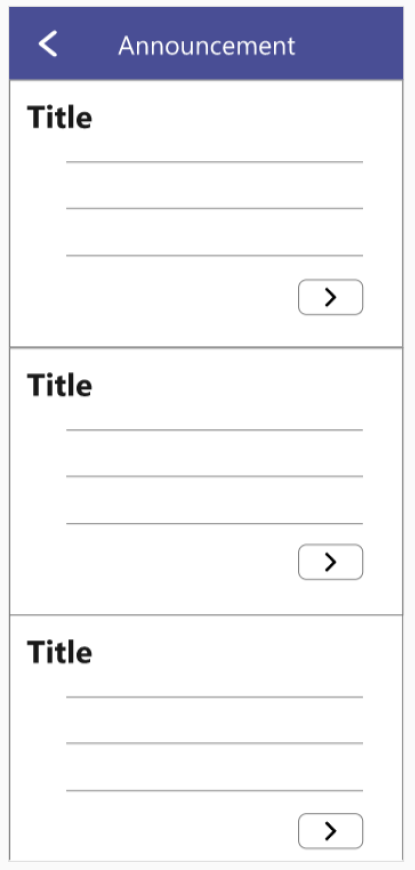
\includegraphics[scale=1]{img/prototype/iter3-proto-5.png}
            \caption{Announcement Screen}
            \label{fig:iter3-proto-5}
          \end{figure}
          \par According to figure \ref{fig:iter3-proto-5}, the application will provide official announcements from the government and
          authorized organizations to the users as a part of user support. This page is expected to be informative,
          genuine, and in real-time so that the users could frequently keep tracks of the latest pandemic updates.
          This implementation is included in the User Support section.
          \begin{figure}[H]
            \centering
            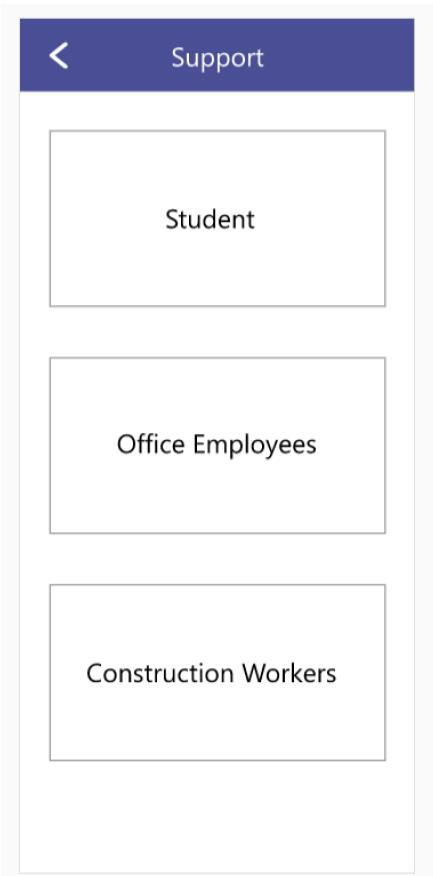
\includegraphics[scale=1]{img/prototype/iter3-proto-6.png}
            \caption{User Support Package Screen}
            \label{fig:iter3-proto-6}
          \end{figure} 
          \par Based on figure \ref{fig:iter3-proto-6}, each respective target audience would receive different support packages from the
          application. In specific, the User Support section would display a wide range of categories
          corresponding to groups of users affected by the pandemic such as students, office employees and
          construction workers. Any other target stakeholders could be included in any further research by
          another team but not in the with last milestone. By tapping on a tab corresponding to the appropriate
          user category, the users could explore valuable assistance packages recommended by the application.
          \begin{figure}[H]
            \centering
            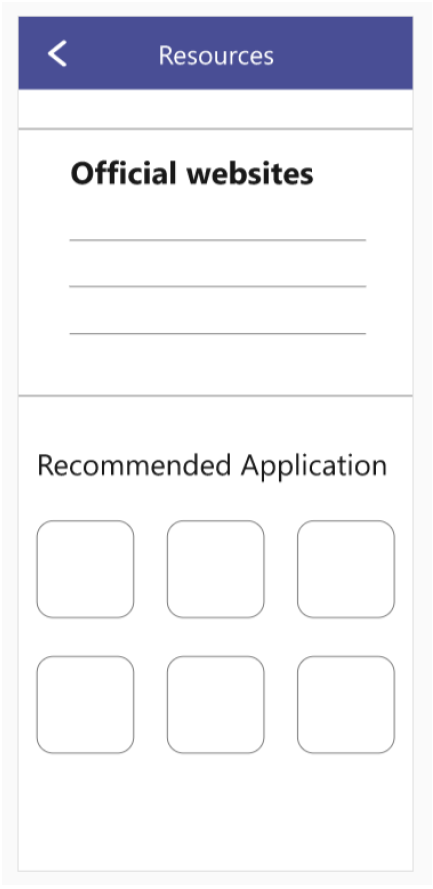
\includegraphics[scale=1]{img/prototype/iter3-proto-7.png}
            \caption{Resource Screen}
            \label{fig:iter3-proto-7}
          \end{figure}
          \par According to figure \ref{fig:iter3-proto-7}, the final step will proceed with the application suggesting useful resources to help users stay healthy physically and mentally. On the Resources page, the users could find essential information about the pandemic such as virus spreading prevention techniques through official websites of government agencies and departments. This section also recommends associated applications that help users to cope with multiple issues during the quarantine.
      \end{enumerate}

  \subsection{Behavioral Design}
    \par Behavioural design is used as a reference and guideline to identify the user behavioural pattern of a
    common majority community towards digital data sharing. This is to study how a user decision may
    be influenced by the common majority community of other people. The study helps us to understand
    how certain design components could be included and designed to increase user participation and
    engagement rate for the application to achieve our product goals. Hence, we integrate the behavioural
    design principles into our proposed solution.

    \subsubsection{Behavioral Modelling}
      \begin{figure}[H]
        \centering
        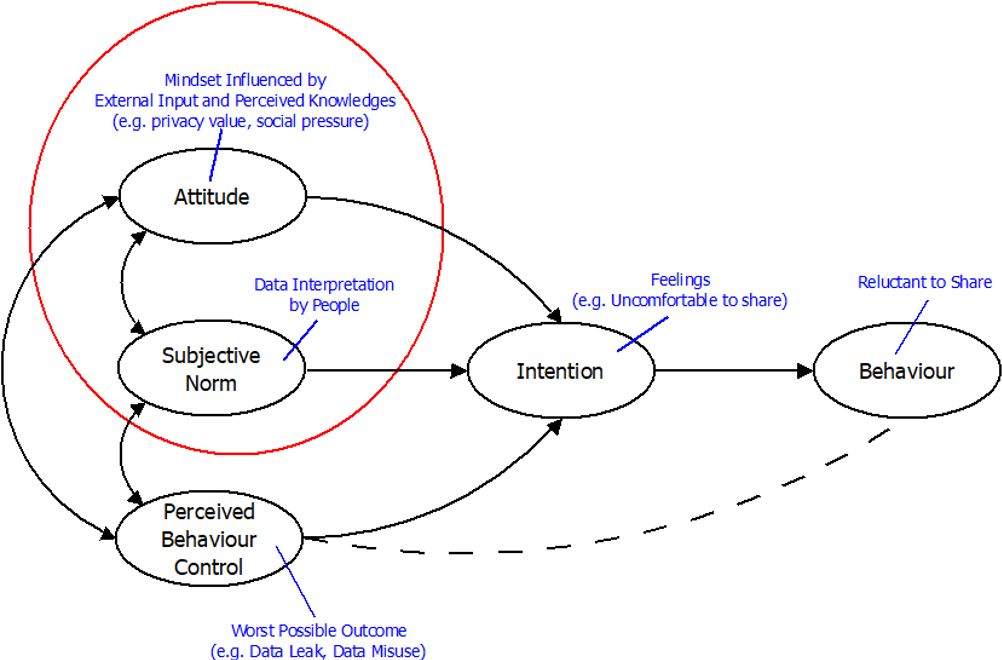
\includegraphics[scale=1]{img/digital-prototype/behavior-model.png}
        \caption{Data Sharing Behavior Model}
        \label{fig:behavior-model}
      \end{figure}
      \par This modelling concept template is borrowed and remodelled from \parencite{Ian8}. The above figure \ref{fig:behavior-model} hows the
      modelling with my notation on how data privacy has been perceived by the general public in current
      times. From the current public behaviour towards a deployed pandemic tracking mobile application,
      most of them are reluctant to share their data and does not find it helpful. This are mostly affected by
      how they perceived the worst possible outcome interpreted by the public eye or based on their own
      knowledge. Hence, it may further influence other peoples' perspective collectively known as
      collective consciousness. This may create norms that are misleading for other people through social
      pressure as well. In other words, we would like to implement some behaviour design principles for
      our application to change the people's attitude that would not be influenced by the current subjective
      norms created for digital data sharing (red circle shown above).
    
    \subsubsection{Behaviour Design Example}
      \begin{enumerate}[a)]
        \item \textbf{Iteration 2}
          \begin{figure}[H]
            \centering
            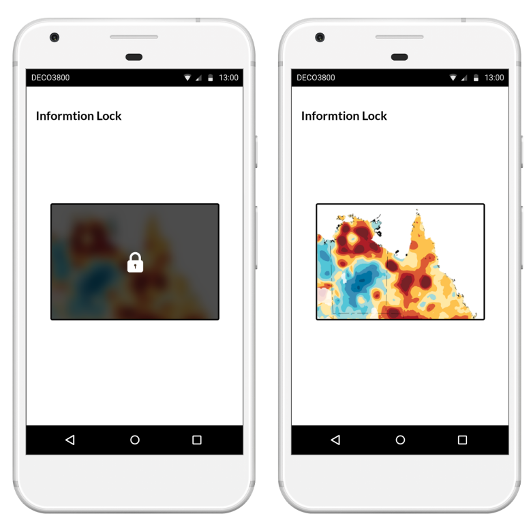
\includegraphics[scale=1]{img/digital-prototype/info-lock-screen.png}
            \caption{Sequential Information Release Example}
            \label{fig:digi-proto-03}
          \end{figure}
      \end{enumerate}

      \par From the above Figure \ref{fig:digi-proto-03}, it displayed an example for the Queensland regional COVID-19 hot zones through a heatmap illustration. The information on left is lock while unlocked on the right. This design had applied a concept called sequential information release. This approach is to limit the disclosure of sensitive data and information to the application users. Moreover, it is equally important and fair to all users when certain users are providing necessary information while others are taking for granted. In such cases, we do not imply consent to any users who are not sharing their information while protecting the privacy of other users who shared their information. Thus, it promotes a scenario of user inducing altruistic behaviour known as reciprocal altruism. In other words, we study the user psychology to create guidelines and implement behaviour design principles into our application which could elevate user experience that could positively impact their mindset of how our application perceive user’s privacy and promote the element of trust to the users.
      \par \textbf{Final Decision}: The team decided to remove the above-mentioned design principle during the end of Iteration 2.
      When aligning our product goals set for Iteration 3, we decided to promote trust using a very different
      approach for the data algorithm (e.g. black box) to store user data, which involves cryptography that
      is not disclosing information without user consent. Hence, the mentioned behavioural design is not
      applicable as there is not information display unless invoked by a scenario (explained in Digital
      Prototyping at Iteration 3). Moreover, sequential release would not be relevant for Iteration 3 as the
      information will need to display in a whole without leaving out any segmented or fragmented
      information. So, it is not possible to user such method to provide data protection for our application.

  \subsection{Usability Testing}
    \par The purpose of usability testing is to evaluate a product through a developed prototype based on the feedbacks collected from the users. It helps to refine user requirements and visual designs of the product throughout the development cycle. Moreover, it focused on how the users interact with the prototype, completes the given tasks, and observe the users during testing. It could collect valuable insights through learning the user’s behaviour and preference from the user testing. Thus, the insights could further improve the prototype for iterative testing sessions.
    \par The prototypes used for testing session are the map simulator and quarantine life simulator. All the participants joined have given their consent for the testing session. The testing is conducted through a link to the prototype through real-time communication via video or phone calls with the participants.
    
    \subsubsection{Retrospective Think Aloud (RTA)}
      \par This technique requires participants to retrace their steps when the session is complete. This technique
      is particularly useful to verbalize the participant thoughts and embed the process into their memory.
      Hence, it could check whether the participants could visualize the contents during memory tracing,
      which indicates how the visual content impression is delivered to them during the session. In other
      word, the user preferences and behaviours would influence how they perceived the simulation
      prototype values and core processes delivered to them.
      \par \textbf{Findings}:
      \begin{itemize}
        \item Map Simulator:
          \begin{itemize}
            \item 4 of 5 participants thinks that the information is insufficient for convincing them from leaving the house.
            \item All participants do not remember the major hot zones after answering it.
          \end{itemize}
        \item Quarantine Life Simulation:
          \begin{itemize}
            \item 3 of 5 participants spent a longer average time testing the quarantine life simulator.
            \item 3 of 5 participants thinks that the quarantine life simulator is a fun-to-play game only.
          \end{itemize}
      \end{itemize}
    
    \subsubsection{Concurrent Probing (CP)}
      \par This testing technique requires participants to work on the tasks given and asking follow-up questions
      when the participants engaged in the session. This technique is suitable to prompt real-time feedbacks
      on upon each task executed, which could directly project their current feelings towards the prototypes.
      In other words, we could understand the user psychology path when carrying out tasks through how
      the application may evoke different feelings towards the user or through the user behaviour in
      performing task on the application. Hence, it creates a minimum threshold on how these
      functionalities could provide its usefulness to increase user retention rate through the testing session.
      \par \textbf{Findings}:
        \begin{itemize}
          \item Map Simulator:
            \begin{itemize}
              \item All members suggested for more travel options. 
              \item 3 of 5 participants suggested to include information as hint when they think it is good and easy to reference for authentication.
            \end{itemize}
          \item Quarantine Life Simulation:
            \begin{itemize}
              \item 2 of 5 participants thinks that the selection rounds could be increase for a more thorough representation of their daily lifestyle.
              \item 4 of 5 participants thinks that the selection categories for each round in the quarantine life simulator are inconsistent. 
            \end{itemize}
        \end{itemize}

    \subsubsection{Insight Summary}
      \begin{enumerate}[a)]
        \item \textbf{Iteration 2}
        \begin{itemize}
          \item Map Simulator:
            \begin{itemize}
              \item More statistical inputs are required to increase user interest and authenticity from verified sources. 
              \item Participants are likely wanting to travel in their own preferred transport only, which the current simulator only display one option travelling by car only. In other words, this may happen to due habits issue or lack of confidence travelling with non-preferred vehicle during this period.
              \item Create important visual components to be more appealing and attractive for developing as a semantic memory during memory encoding (Behavioural design principles).
              \item Providing minor support as guidelines such as nudge could its memory point for user impression.
            \end{itemize}
          \item Quarantine Life Simulation:
            \begin{itemize}
              \item Create selection within the category in each round for better memory tracing.
              \item Providing selection pictures that are more approximate to local culture and habits accordingly.
              \item More in-depth analysis for the daily summary should be carried out with the prompted input.
              \item Participants tends to spend more time for recalling and retracing memory with the selection pictures each round, indicating the significant values as an additional component to increase retention rate.
            \end{itemize}
        \end{itemize}
      \end{enumerate}